\documentclass[10pt]{beamer}

\usepackage{amsfonts}
\usepackage{subfiles}
\usepackage[T2A]{fontenc}
\usepackage[utf8]{inputenc}
\usepackage[english, russian]{babel}

\usepackage{amsmath, amsfonts, amssymb, amsthm, mathtools, mathrsfs}
\usepackage{wasysym, dsfont}
\usepackage{graphicx}
\usepackage{float}
\usepackage{wrapfig}
\usepackage{subcaption}
\usepackage{multirow}
\usepackage{caption}
\usepackage{subcaption}
\usepackage{xcolor}
% \usepackage{subfigure}

\usepackage{multicol}
\DeclareMathOperator*{\argmax}{\arg\!\max}
\DeclareMathOperator*{\argmin}{\arg\!\min}
\DeclareMathOperator{\sr}{sr}
\DeclareMathOperator{\rank}{rank}
\DeclareMathOperator{\tr}{tr}

\mode<presentation>
{
	\usetheme{boxes}
	\beamertemplatenavigationsymbolsempty{}
	
	\setbeamertemplate{footline}[page number]
	\setbeamersize{text margin left=1em, text margin right=1.5em}
}
\newcommand\blfootnote[1]{%
	\begingroup
	\renewcommand\thefootnote{}\footnote{#1}%
	\addtocounter{footnote}{-1}%
	\endgroup
}
\newcommand\FontUP{\fontsize{12}{12}\selectfont}


\title[]{Анализ выразительности и обобщающей способности LoRA}

\author{Охотников Н.В.\\ Научный руководитель: Грабовой А.В. к.ф.-м.н.}


\institute{МФТИ}
\date{2026}

\begin{document}

\begin{frame}
  \titlepage{}
\end{frame}


\begin{frame}
    % \frametitle{Introduction}
    \vfill
    \begin{block}{Цель}
        Предложить улучшение теоретических оценок выразительности и обобщающей способности нейронных сетей, обучаемых методом LoRA 
    \end{block}
    \vfill
    \begin{block}{Проблема}
        Известные оценки не учитывают неявные ограничения процесса оптимизации при обучении с LoRA
    \end{block}
    \vfill
    \begin{block}{Предлагается}
        Использовать эмпирическое ограничение на stable rank матриц адаптеров. Уточнить оптимальное решение задачи аппроксимации матрицы матрицей меньшего ранга с учетом дополнительного ограничения на stable rank.
        Использовать PAC-Bayes фреймворк для улучшения оценки обобщающей способности.
    \end{block}
\end{frame}


\begin{frame}
    \frametitle{Аппроксимация отдельной матрицы}
    \vspace{-0.8cm}
    $$\text{Stable rank матрицы } A \text{ : } ~ sr(A) = \frac{\|A\|_F^2}{\|A\|_{op}^2} = \frac{\sum_i \sigma_i^2(A)}{\sigma_1^2(A)}$$
    $$\mathcal{M}_{R,S}^{d,d} \subset \mathbb{R}^{d\times d},~ \forall A \in\mathcal{M}_{R,S}^{d,d}:~ rank(A) \leqslant R, sr(A) \leqslant S$$
    Пусть $A\in \mathbb{R}^{d\times d}$, $A_R = \sum_{i=1}^R \sigma_i u_i v_i^T$ - оптимальная (по норме Фробениуса) аппроксимация $A$ матрицей ранга $R$ (из сингулярного разложения)

    Пусть $\hat{A} \in \mathcal{M}_{R,S}^{d,d}$ такова, что  $\inf\limits_{\tilde{A}\in \mathcal{M}_{R,S}^{d,d}}\|A - \tilde{A}\|_F^2 = \|A - \hat{A}\|_F^2$

    \begin{block}{Лемма 1 [Охотников, 2026]}
        \vspace{-0.5cm}
        $$\hat{A} = \sum_{i=1}^R \hat{\sigma_i} u_i v_i^T, \quad \text{где }\hat{\sigma_i} = \sigma_i, \text{ если }sr(A_R) \leqslant S, \text{ иначе: }$$
        \vspace{-0.3cm}
        $$\hat{\sigma}_1 = \tfrac{\sigma_1 + \sqrt{S-1}\sqrt{\sum_{j=2}^R\sigma_j^2}}{S},\quad \hat{\sigma}_i = \gamma \sigma_i ~ (i \geqslant 2), \;\gamma = \tfrac{\sqrt{S-1}\hat{\sigma}_1}{\sqrt{\sum_{j=2}^R\sigma_j^2}}$$
        
        Причём $\|A - \hat{A}\|_F^2 = \sum_{i=R+1}^{D}\sigma_i^2 + \Delta_S$, ~ $\Delta_S = 0$, если $\sr(A_R) \leqslant S$, иначе:

        \hspace{3cm} $\Delta_S = \frac{1}{S}\big(\sqrt{\sum_{i=2}^R\sigma_i^2} - \sqrt{S-1}\sigma_1\big)^2$
    \end{block}
\end{frame}


\begin{frame}
    \frametitle{Выразительность в полносвязной сети}
    % \vspace{-0.3cm}
    \begin{block}{Обозначения}
        $\text{целевая FNN  }~~ \overline{f}:=FNN_{\overline{L},D}(.;(\overline{W}_l)_{l=1}^L, (\overline{b}_l)_{l=1}^L), $ - хотим приблизить \\
        $\text{предобученная FNN }~~ f_0:= FNN_{L,D}(.;(W_l)_{l=1}^L, (b_l)_{l=1}^L),$\\
        $\text{предобученная с адаптером FNN }~~ f:=FNN_{L,D}(.;(W_l + \Delta W_l)_{l=1}^L, (\hat{b}_l)_{l=1}^L)$\\
        $b_l, \overline{b}_l, \hat{b}_l \in \mathbb{R}^D$, $W_l, \overline{W}_l, \Delta W_l \in \mathbb{R}^{D\times D}$, $\Delta W_l = A_l B_l$, где $A_l\in \mathbb{R}^{D\times R}$ и $B_l\in \mathbb{R}^{R\times D}$ и $R\leqslant D$ -- ранг LoRA.
    \end{block}
    \begin{block}{Теорема 1 (Выразительность LoRA для FFN) [Охотников, 2026]}
        Пусть $x\in \mathbb{R}^d$ случайный вектор с ковариационно матрицей $\Sigma = \mathbb{E}[xx^T]$.
        Пусть $E_l = \overline{W}_l - W_l$. Пусть $E_{l,R}$ оптимальная аппроксимация ранга $R$ с $\sigma_{l,1} \geqslant \dots \geqslant \sigma_{l,R}$. Пусть $\hat{b}_l = \overline{b}_l$. Тогда  $\exists \{\Delta W_l\}_{l=1}^L \subset \mathcal{M}_{R,S}^{D,D}$ такие что:
        \vspace{-0.3cm}
        $$ \mathbb{E} \| f(\mathbf{x}) - \overline{f}(\mathbf{x}) \|_2 \leqslant \beta \sum_{l=1}^L \left( \prod_{k=l+1}^L \| \overline{W}_k \|_2 \right) \mathcal{T}_l, ~\text{где} $$
        \vspace{-0.3cm}

        $ \beta = \max_{i \in [L]} \left( \left( \prod_{j=1}^i \|\overline{W}_j\| \right) \sqrt{\text{tr}(\Sigma)} + \sum_{j=1}^i \left( \prod_{k=j+1}^i \|\overline{W}_k\| \right) \|\overline{b}_j\| \right) $\\
        и $ \mathcal{T}_l = \sqrt{ \sum_{j=R+1}^D \sigma_{l,j}^2 + \Delta_{S,l} }, ~~\text{где }$
        
        $\Delta_{S,l} = \frac{1}{S}\Big(\sqrt{\sum_{j=2}^R\sigma_{l,j}^2} - \sqrt{S-1}\sigma_{l,1}\Big)^2  \text{если } \sr(E_{l,R}) > S, ~~  \text{иначе } 0$
    \end{block}
\end{frame}


\begin{frame}
    \frametitle{Выразительность в архитектуре transformer}
    \vspace{-0.3cm}
    \begin{block}{Обозначения}
        Трансформер $L$ блоков -- $H$-головый self-attention + 2-слоный FFN, без dropout/нормализаций, но со skip connection \\
        Целевая сеть $\overline{f}$, замороженная $f_0$, адаптированная $f$ (LoRA на всех $Q,K,V,O$, обоих слоях FFN).\\
        $\mathcal{T}(G) = \sqrt{\sum_{i=R+1}^{D}\sigma_i^2(G) + \Delta_S(G)}$ -- ошибка для матрицы $G$ из \textbf{Леммы 1}.
    \end{block}
    \vspace{-0.2cm}
    \begin{block}{Теорема 2(Выразительность LoRA для Transformer) [Охотников, 2026]}
        \vspace{-0.2cm}
        Существует набор матриц адаптеров $\{\Delta W\}\subset \mathcal{M}_{R,S}^{D,D}$ с SR $\leqslant S$ такой, что
        \vspace{-0.2cm}
        $$\mathbb{E}\|f(x) - \overline{f}(x)\|_F \leqslant \beta\sum_{l=1}^{L}\Big(\prod_{k=l+1}^L \gamma_k\Big)\mathcal{D}_l$$
        $\bullet$ $\gamma_k$: константа Липшица целевого блока $k$ по входу (через FFN + MHA)\\
        $\bullet$ $\mathcal{D}_l = \mathcal{T}_{2,l} + \|\overline{W_{2,l}}\|\mathcal{T}_{1,l} + \|\overline{W_{2,l}}\|\|\overline{W_{1,l}}\|\sum_h \mathcal{D}_{att,l}^h$ (ошибки FFN + attention)\\
        $\bullet$ $\mathcal{D}_{att,l}^h$: ошибка головы $\propto \mathcal{T}_{O},\mathcal{T}_{V},\mathcal{T}_{Q},\mathcal{T}_{K}$
    \end{block}
\end{frame}


\begin{frame}
    \frametitle{Оценка обобщающей способности}
    \vspace{-0.2cm}
    \begin{block}{Обозначения}

        Полносвязная сеть глубины $T$, ширины $d$ $f_W$, с 1-липшицевой функцией активации $\sigma(.)$, $\sigma(0)=0$, LoRA на каждом слое $\Delta W_t = B_t A_t^T$, $W_t = W_{0,t} + \Delta W_t$. $\|\Delta W_t\|_{op} \leqslant \Lambda_t$, $\sr(\Delta W_t) \leqslant S_t$, пусть вход $x_i:$ $\|x_i\|_2 \leqslant B_x$
        \vspace{-0.15cm}
        $$\text{Margin: } m(f_W(x), y) = f_W(x)_y - \max_{j \neq y} f_W(x)_j$$
        \vspace{-0.5cm}
        $$L_\gamma(W) = \mathbb{P}_{(x,y)}[m(f_W(x), y) \le \gamma], \;\; \widehat{L}_\gamma(W) = \tfrac{1}{N}\sum_{i=1}^N \mathbb{I}[m(f_W(x_i), y_i) \le \gamma]$$

        $L_0$ -- истинный риск. Generalisation gap $G = \sup\limits_{f_W} |L_0 - \hat{L_0}|$
    \end{block}

    \vspace{-0.2cm}
    \begin{block}{Теорема 3 (Обобщающая способность LoRA) [Охотников, 2026]}
        $\forall \gamma > 0$ и любых $\Delta W_t$, удовлетворяющего указанным выше условиям, с вероятностью не менее $1-\delta$ по выбору обучающей выборки размера $N$:
        \vspace{-0.1cm}
        $$L_0(W) \leqslant \widehat{L}_\gamma(W) + \mathcal{O}\!\left(\!\sqrt{\tfrac{B_x^2 T^2 (d + \ln(TN)) \left( \prod_{t=1}^T \bar{\beta}_t^2 \right) \sum_{t=1}^T \frac{\Lambda_t^2 S_t}{\bar{\beta}_t^2} + \log(N/\delta)}{\gamma^2 N}}\right)$$

        \vspace{-0.4cm}

         $\mathcal{O}(\sqrt{S/N})$ в отличие от наилучшего ранее известного $\mathcal{O}(\sqrt{r/N})$.
    \end{block}
\end{frame}


\begin{frame}
    \frametitle{Эксперимент}

    \textbf{Архитектура:} MLP ширина $D=128$, глубина $L=10$. Схема <<учитель--ученик>>.

    \textbf{Инициализация:} одинаковые веса ученика и учителя, далее сдвиги $\Delta W_l$ для весов учителя с разным SR

    \textbf{Контроль SR:} $U \operatorname{diag}(\sigma) V^T$ -- SVD случайной матрицы, далее $\sigma_1 \rightarrow \sigma_1 \cdot c_i$, где $c_1$--$c_8 = \{1.0, 1.5, 2.0, 3.0, 5.0, 8.0, 12.0, 20.0\}$

    \textbf{Данные:} $x\sim \mathcal{N}(0, I) \rightarrow \text{ учитель } + \varepsilon \rightarrow y$ , $N_{\text{train}}=2048$, $N_{\text{val}}=10240$. 

    \textbf{LoRA:} ранги $r \in \{4, 6, 8, 12, 16, 24, 32, 48, 64, 96, 128\}$ + полное дообучение

    \textbf{Обучение:} AdamW, 200 эпох, $lr=10^{-3}$.

    \textbf{Метрики:} Generalization gap = loss(valid) $-$ loss(train). Средний stable rank $\overline{\sr}$ адаптеров.

\end{frame}


\begin{frame}
    \frametitle{Результаты эксперимента}
    \vspace{-0.3cm}
    \centering
    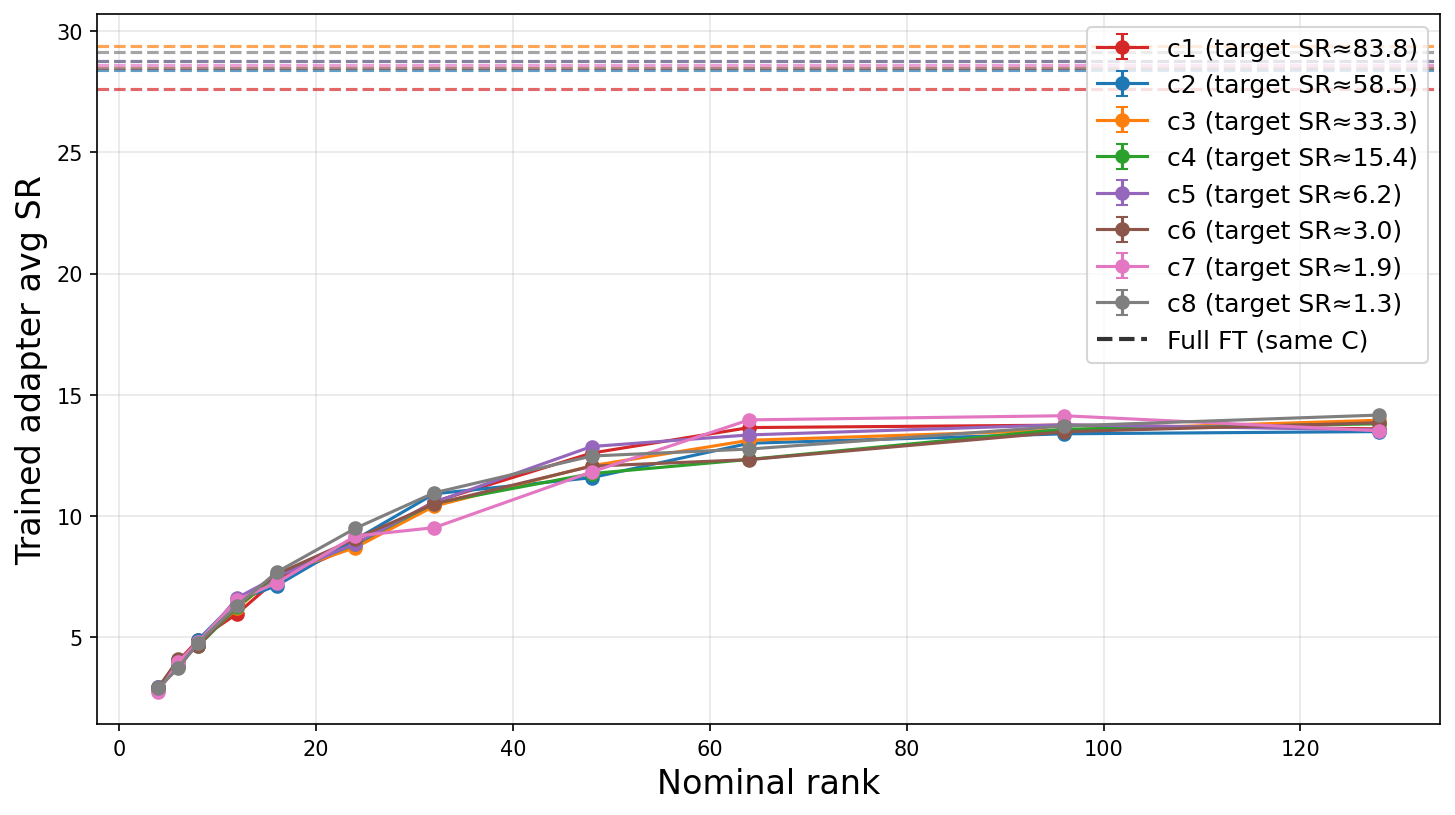
\includegraphics[width=0.55\textwidth]{../figures/regression_trained_sr_vs_nominal_rank.png}

    \vspace{0.5cm}
    \begin{columns}
        \begin{column}{0.53\textwidth}
            \centering
            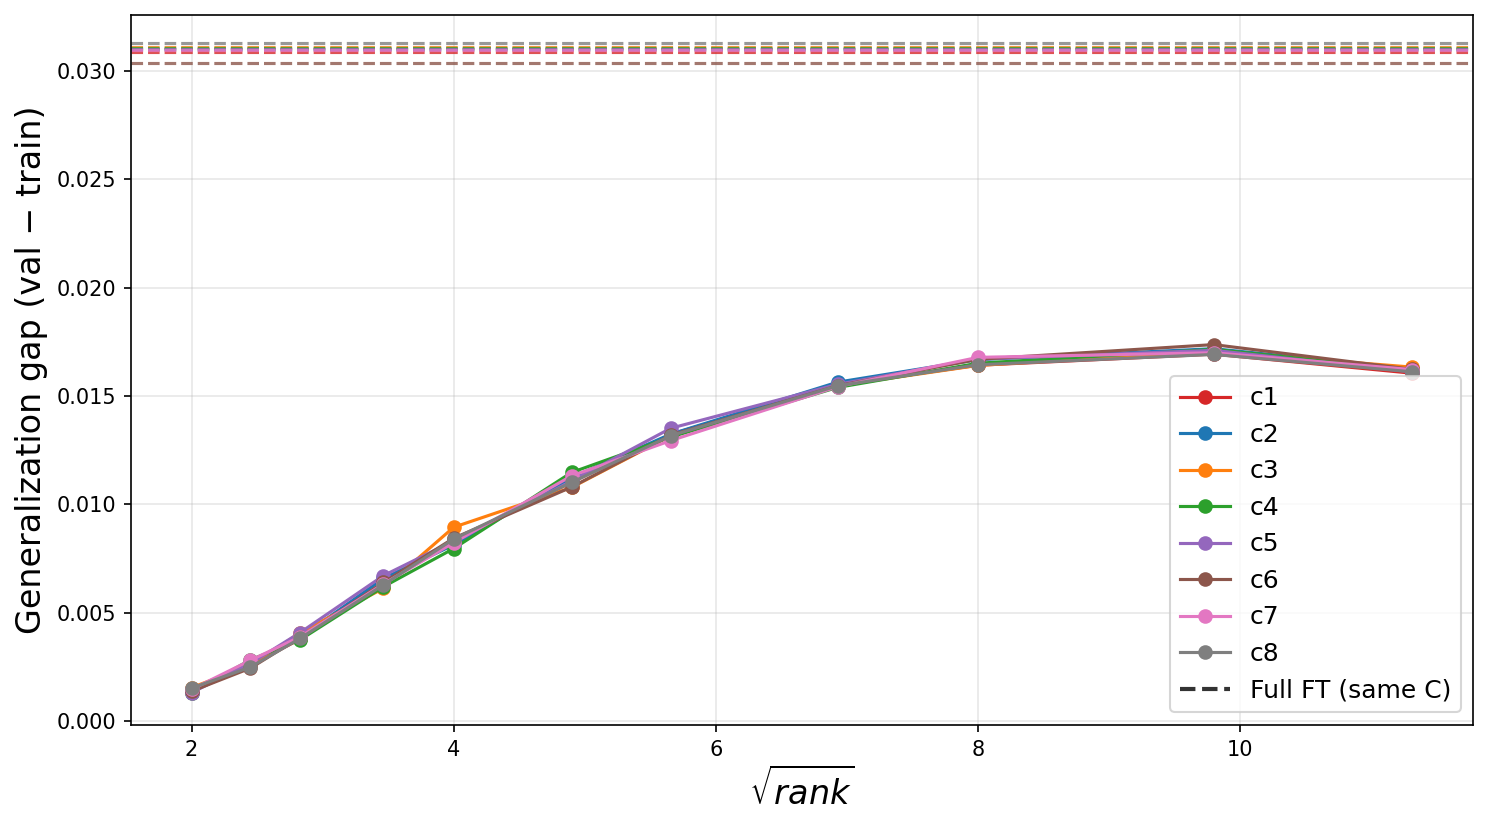
\includegraphics[width=\textwidth]{../figures/regression_gen_gap_vs_sqrt_rank.png}
        \end{column}
        \begin{column}{0.53\textwidth}
            \centering
            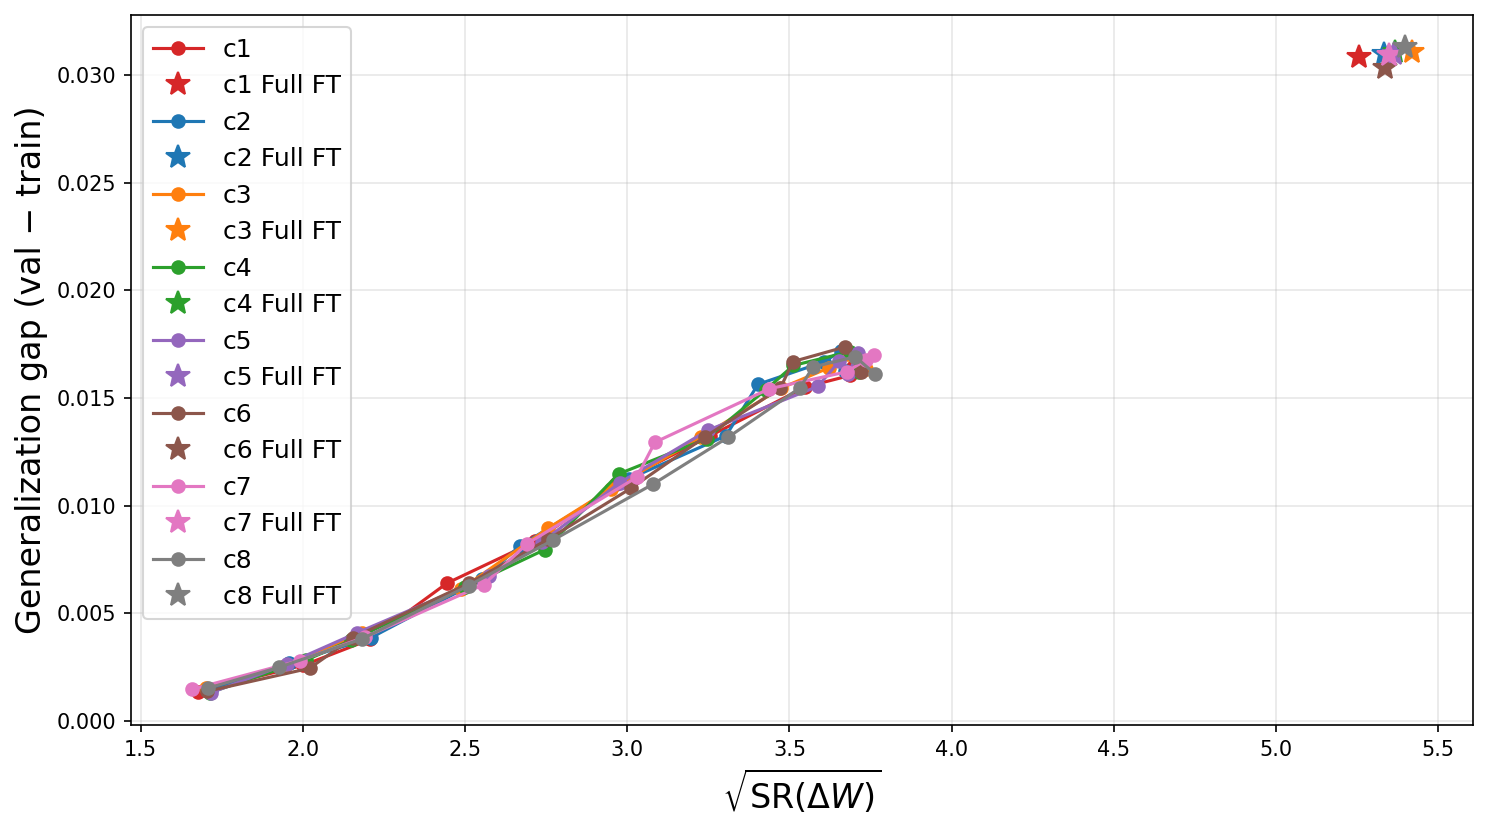
\includegraphics[width=\textwidth]{../figures/regression_gen_gap_vs_sqrt_trained_sr.png}
        \end{column}
    \end{columns}

\end{frame}


\begin{frame}
    \frametitle{Выносится на защиту}
    \begin{enumerate}
        \item Доказана лемма для оптимальной аппроксимации матрицы матрицей c рангом $\leqslant R$ и stable rank $\leqslant S$
        \item Уточнены границы выразительности LoRA для FNN и Transformer с учётом stable rank
        \item Усилена верхняя оценка на generalisation gap для LoRA с $\mathcal{O}(\sqrt{R/N})$ до $\mathcal{O}(\sqrt{S/N})$
        \item Экспериментально показано, что $\propto \sqrt{S}$ лучше чем $\propto \sqrt{R}$ приближает динамику generalisation gap при изменении гиперпараметров
        \item Экспериментально показано, что stable rank является лучшим чем алгебраический ранг индикатором для масштабирования обобщающей способности и выразительности
    \end{enumerate}
\end{frame}




\end{document}
